This section will cover which features were modified and added to AirSim to reach the desired behaviour. Each section will look at the challenges faced and discuss previous approaches. The sections will also explain which bits of existing code the feature is based off, or if the feature was written from scratch.

\subsection{Multiple Entities}
The first modification to be made to the simulator was to make sure that it could handle multiple agents. This was an essential step as the simulator could not be used if having several agents at once was not possible. Currently, the simulator is primarily designed for one agent. After initial research, the simulator should have been able to handle two vehicles if this was added to the startup configuration. However, this did not work in Unity. 

The first step was to modify the existing APIs so that the vehicles could be accessed individually. To do this, all vehicles were added to a global list. Each vehicle was also given a unique identifying name. The next step was to add an argument to each API specifying the vehicle.  When a vehicle API was called, Unity would first iterate over the map looking for the corresponding vehicle. Once the entity was found Unity would then forward the API request to that vehicle. This change had to be made throughout AirSim tracing the call from the user interaction in Python to Unity. 

The main challenges faced when doing this was originally trying to adapt the configuration file. As this had not been properly implemented in Unity yet, time was spent trying to debug this issue. Eventually, it was discovered that adding the vehicles manually to the scene before starting would be easier. 

Currently, if two vehicles are given the same name the second vehicle will spawn, but the API calls will only be redirected to the first vehicle. This can easily be changed so that either both entities should behave in the same way, or that the second entity does not spawn. This behaviour however was seen as unimportant and have been left out for the time being. 
 

\subsection{Spawning Entities at Runtime}

\subsection{Video feed} \label{06:VideoFeed}

\begin{figure}[h]
    \centering
    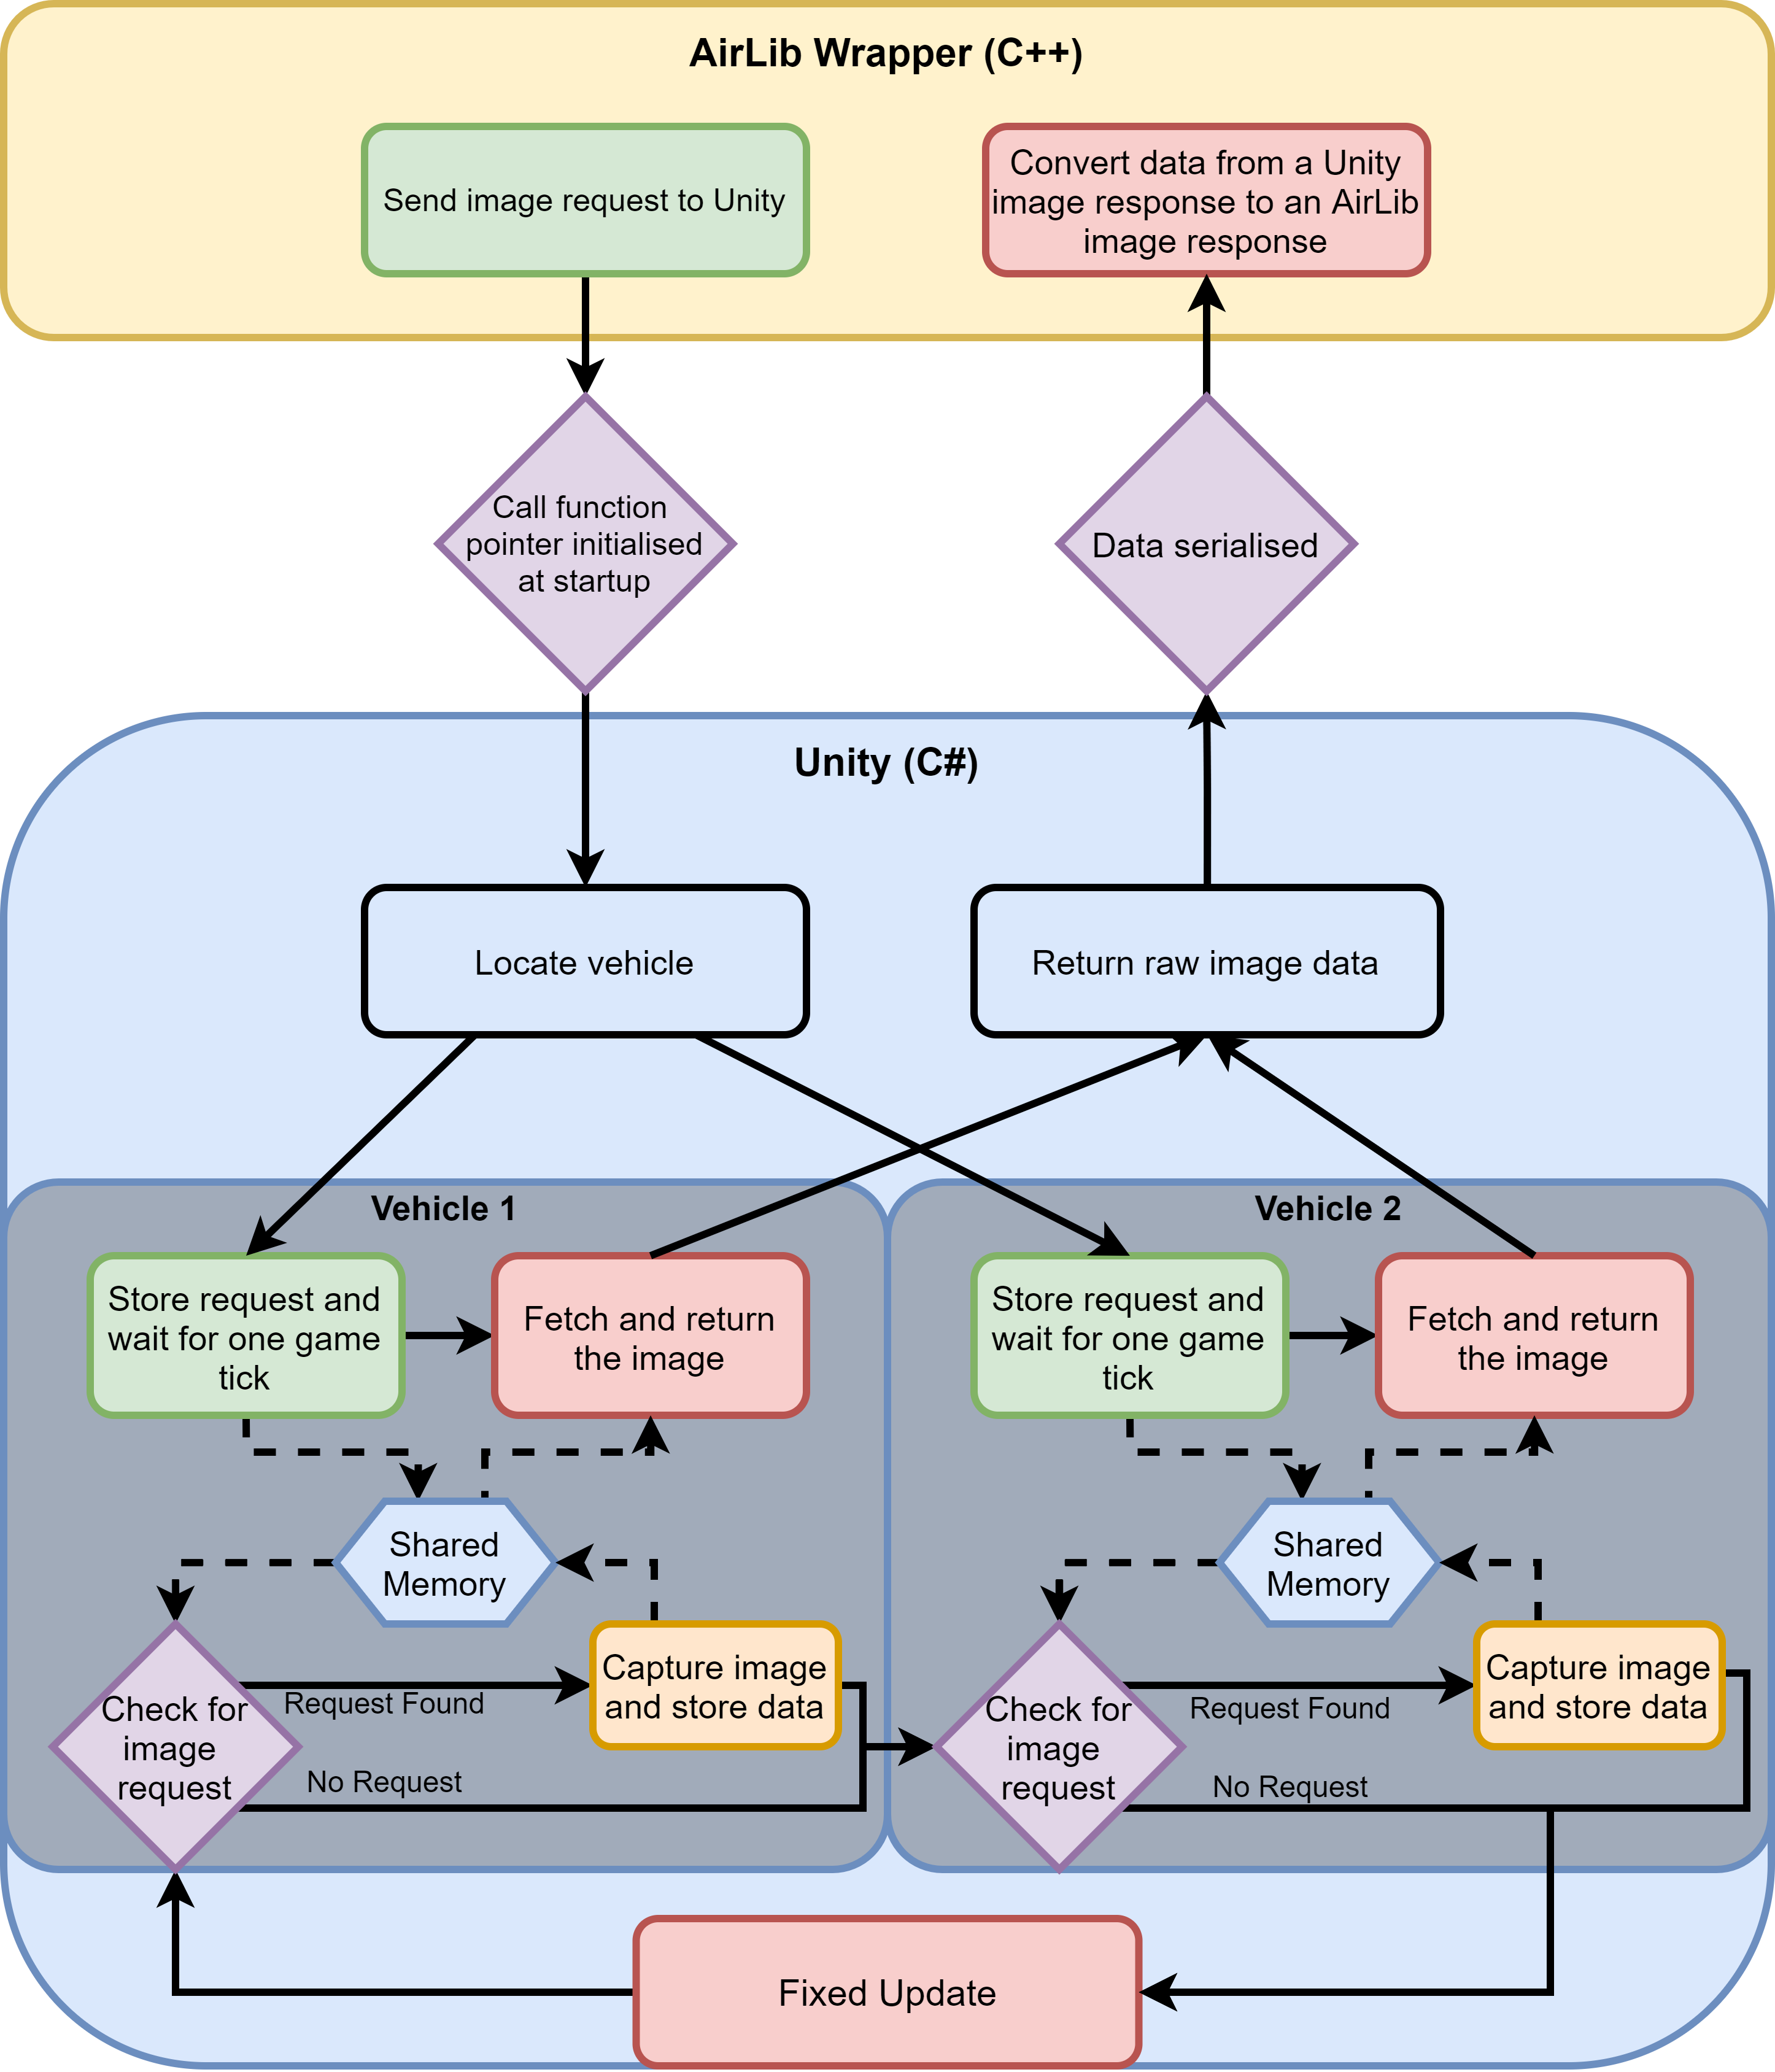
\includegraphics[width=1.0\textwidth]{06_Implementation/00_AirSim/Diagrams/imagecapture.png}
    \caption{} \label{06:imageCapture}
\end{figure}

\begin{figure}[h]
    \centering
    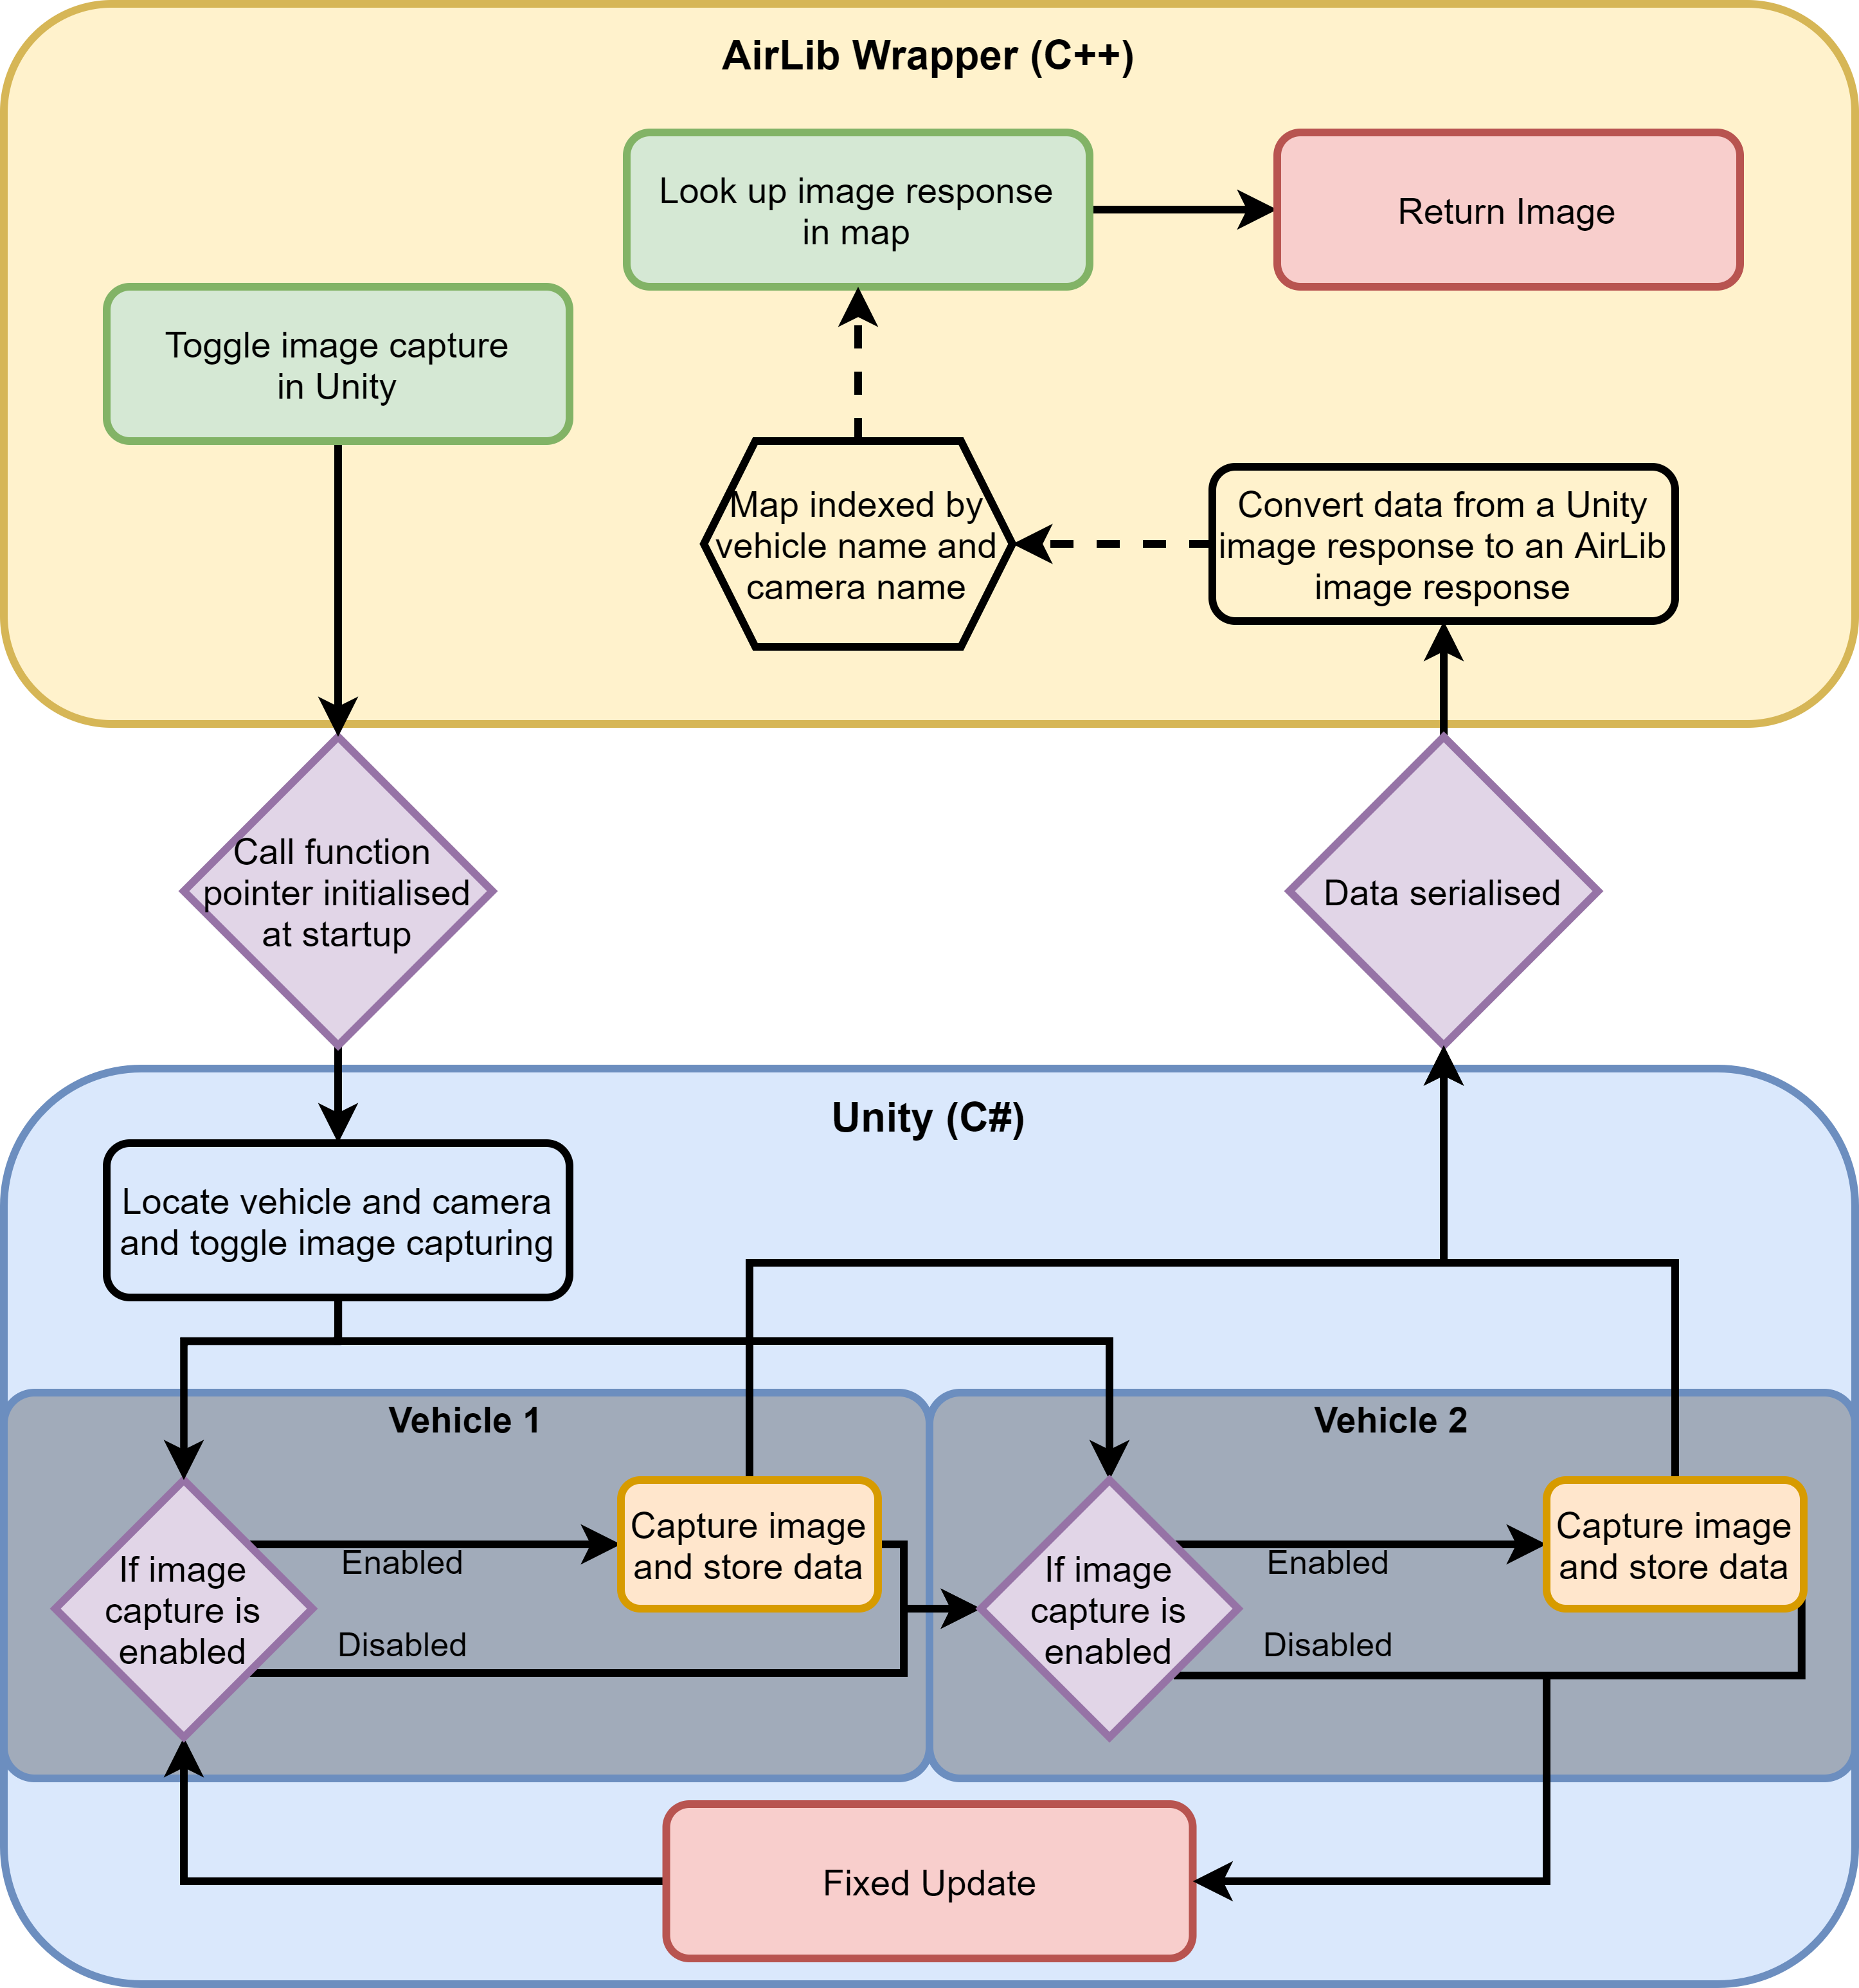
\includegraphics[width=1.0\textwidth]{06_Implementation/00_AirSim/Diagrams/imagecaptureUpdated.png}
    \caption{} \label{06:imageCaptureUpdated}
\end{figure}

\subsection{Adding Pedestrians}
%https://www.mixamo.com/


\subsection{Additional APIs}

\begin{figure}[h]
    \centering
    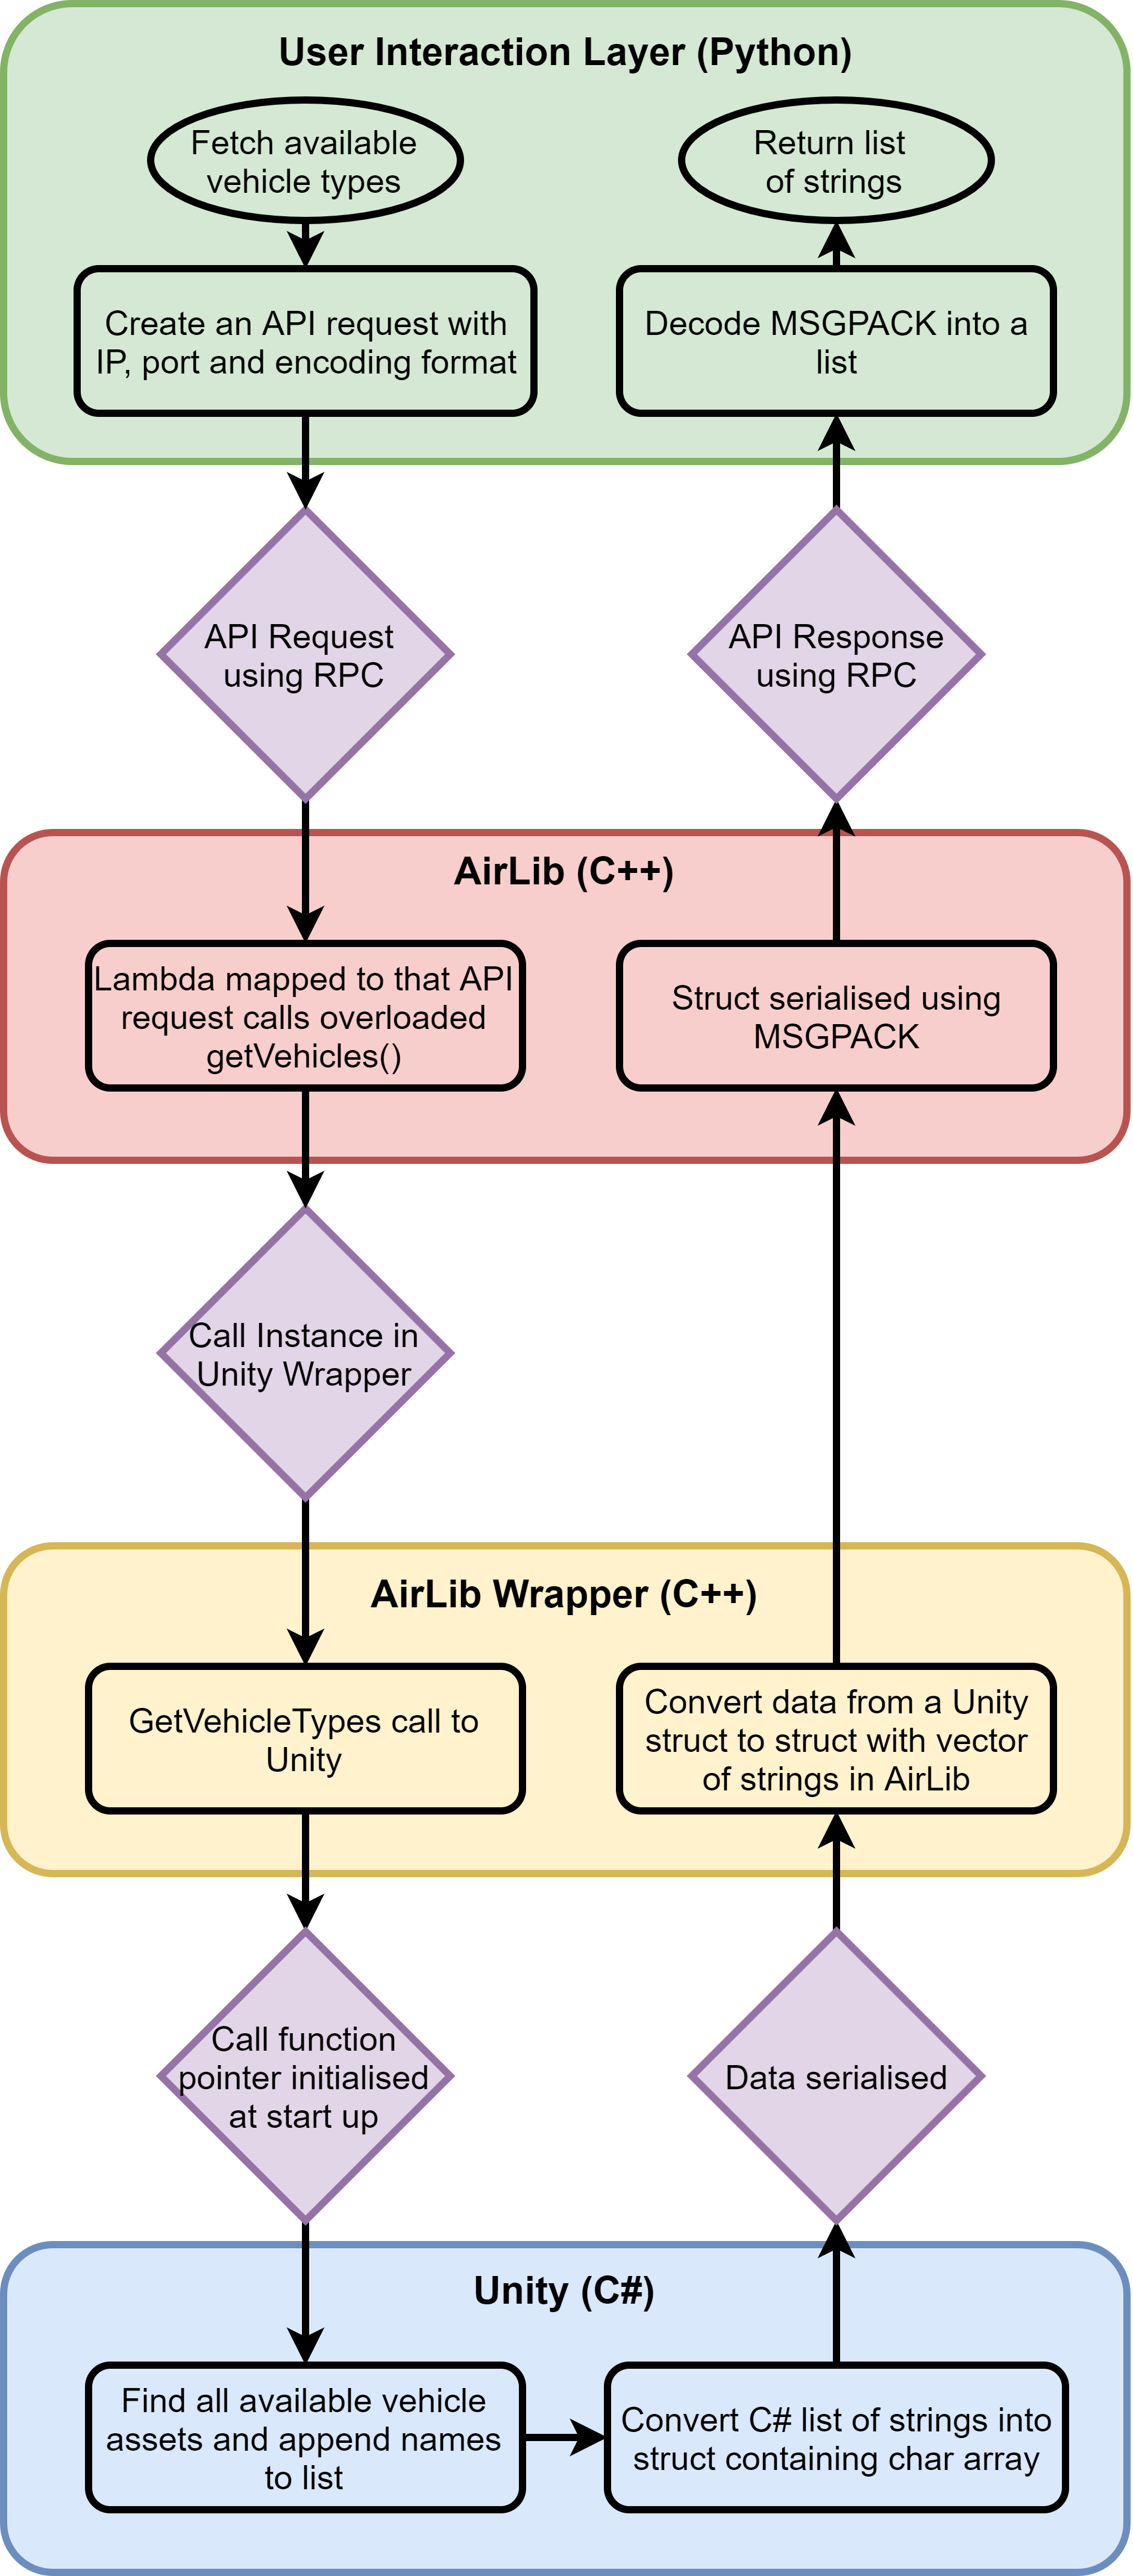
\includegraphics[width=0.6\textwidth]{06_Implementation/00_AirSim/Diagrams/stringArray.png}
    \caption{High-level overview of the API that fetches available vehicle types. For APIs that require arguments, these will be encoded and added to the API request. The main change between different API requests is what happens in Unity.} \label{06:stringList}
\end{figure}

\subsection{Minor Features added}
This section will briefly list other features added. 
%freecam and change between vehicles and entities
%Added global print from server - First thing to be added to get used to the codebase. 
%Rebuild script?




% Why did this not already exist
% •	Used to use config file. Not needed before.
% What changes had to be made
% •	Adding a new API to spawn vehicles, with position, rotation and name as arguments. 
% •	Server is connected to vehicle. Start server without vehicle
% How was the change made.
% •	Add APIs like diagram to spawn vehicles. 
% Challenges faced.
% •	Function pointers not bound by that point in time. Move vehicle spawning. 
% •	Issues with the threading

% Any limitations or known issues?

